\setAuthor{}
\setRound{lõppvoor}
\setYear{2020}
\setNumber{G 5}
\setDifficulty{5}
\setTopic{TODO}

\prob{Gloobus}
\begin{wrapfigure}{r}{0.35\textwidth}
  \vspace{-25pt}
  \begin{center}
  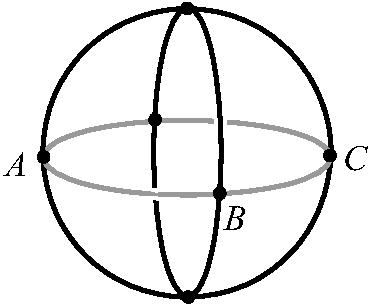
\includegraphics[scale=0.7]{2020-v3g-05-yl.pdf}
  \end{center}
  \vspace{-25pt}
\end{wrapfigure}
Sandral oli igav ja ta leidis vanatädi sahtlist kolm traadijuppi.
Ta ühendas need võrdsete raadiustega rõngasteks ning ehitas  huvi pärast gloobuse,
nii nagu joonisel näidatud. Rõngad jaotasid üksteist võrdselt neljaks ning nende
lõikepunktides olid sõlmed. Traadid olid ühtlase joontakistusega ning Sandra mõõtis
oommeetriga üksikute traadijuppide takistusteks $R_1=\SI{4}\Omega$ (joonisel hall
rõngas) ja $R_2=\SI{8}\Omega$ (joonisel mustad rõngad). Mis oleks mõõdetav takistus \\
\osa~klemmide \emph{A} ja \emph{C} vahel;\\
\osa~klemmide \emph{A} ja \emph{B} vahel.\\


\hint

\solu
\osa Pöördsümmeetria tõttu on näha, et väljundklemmide \emph{A} ja \emph{C} vahele jäävatel sõlmedel on kõigil sama potentsiaal. Seega võib need neli sõlme kokku ühendada ja saame kaks järjestikust neljatakistilist rööbitiühendust:\\
\begin{center}
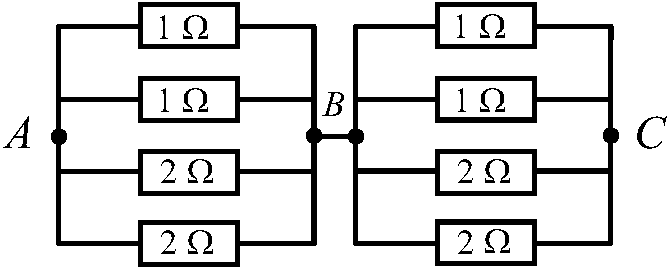
\includegraphics[scale=0.8]{2020-v3g-05-yl1.pdf}\\
\end{center}
Takistus \emph{A} ja \emph{C} vahel on seega: $$2 \cdot \frac{1}{\displaystyle{2 \cdot \frac{1}{2} + 2 \cdot \frac{1}{1}}} \,\, \SI{}\Omega=\frac{2}{3} \, \SI{}\Omega.$$

\osa \emph{Variant 1:} Kerast on võimalik saada ekvivalentne skeem:\\
\begin{center}
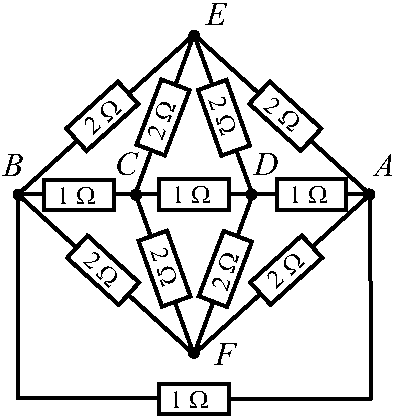
\includegraphics[scale=0.8]{2020-v3g-05-yl2.pdf}\\
\end{center}
kus on lisatud veel sõlmede tähised \emph{D}, \emph{E} ja \emph{F}. Kuna sõlmedel \emph{E} ja \emph{F} on sama potentsiaal, saame need kokku ühendada sõlmeks \emph{O}, nagu järgneval skeemil. Sel juhul on sõlmega \emph{O} ühendatud neli takisti paari, kus üks paar, mis koosneb kahest rööbiti ühendatud 2-oomisest takistist, annab kokku tavalise 1-oomise takisti:
\begin{center}
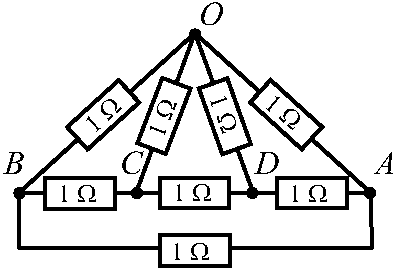
\includegraphics[scale=0.8]{2020-v3g-05-yl3.pdf}\\
\end{center}
Nüüd saame tänu sümmeetriale sõlme \emph{O} poolitada:
\begin{center}
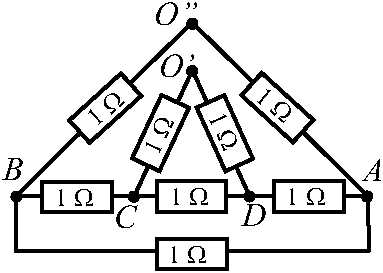
\includegraphics[scale=0.8]{2020-v3g-05-yl4.pdf}\\
\end{center}
Uue skeemi järgi arvutame \emph{A} ja \emph{B} vahelise takistuse:

$$ \frac{1}{\frac{1}{\displaystyle{\frac{1}{\frac{1}{2}+1} + 1 \cdot 2}}+\frac{1}{2}  + 1} \,\, \SI{}\Omega =\frac{8}{15} \, \SI{}\Omega.$$

\emph{Variant 2:} Muutes \emph{C} ja \emph{D} vahelise takistise kaheks 0,5-oomiseks jadamisi takistiks ja öeldes, et \emph{C} ja \emph{D} keskel on uus punkt \emph{O}, siis on \emph{E},\emph{F} ja \emph{O} sama pingega ning need saab ühendada üheks punktiks. Sellega taandub skeem jadamisi ja rööbiti ühendusteks:
\begin{center}
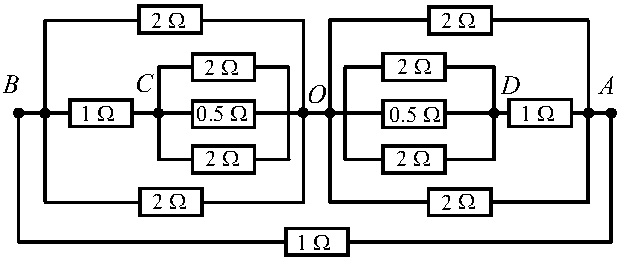
\includegraphics[scale=0.9]{2020-v3g-05-yl5.pdf}\\
\end{center}
mille kogutakistuse välja arvutamisel saame samuti $\frac{8}{15} \, \SI{}\Omega$.
\probend